\chapter{PHƯƠNG PHÁP ĐỀ XUẤT}

\section{Tổng quan về mô hình được đề xuất}
Với đầu vào là một ảnh $I$, mạng MixVPR sẽ tạo ra một tập giá trị mã hóa, đại diện cho ảnh. Giá trị này sẽ được dùng để tìm kiếm ảnh $I'$ có độ tương đồng cao trong tập dữ liệu. Sau khi đã tìm được ảnh tham khảo từ tập dữ liệu, mô hình tương quan 2D-2D của Map-free Relocalization sẽ được sử dụng để xác định độ lệch về vị trí và góc quay giữa ảnh $I$ và $I'$. Cuối cùng, tọa đô tuyệt đối của ảnh $I$ trong không gian sẽ được xác định từ độ lệch và vị trí tuyệt đối của ảnh $I'$.

Như một phương pháp hồi quy vị trí tương đối bình thường, mô hình được đề xuất sẽ bao gồm hai bộ phận chính là bộ phận truy xuất ảnh và bộ phận hồi quy vị trí tương đối dựa trên cặp ảnh. Cụ thể hơn:
\begin{itemize}
    \item Bộ phận truy xuất ảnh sẽ sử dụng mô hình được đề xuất trong bài báo nghiên cứu MixVPR.
    \item Bộ phận hồi quy vị trí tương đối dựa trên cặp ảnh gồm ảnh truy vấn và ảnh tham khảo sẽ sử dụng mô hình tương quan 2D-2D được đề xuất trong bài báo nghiên cứu Map-free Relocalization.
\end{itemize}

\subsection{MixVPR \cite{alibey2023mixvpr}}
\subsubsection*{Ý tưởng đằng sau mô hình}
MixVPR là một phương pháp tổng hợp toàn diện sử dụng Feature Map trích xuất từ một mô hình cơ sở đã được huấn luyện trước đó. MixVPR sẽ lần lượt kết hợp thông tin toàn cục vào mỗi Feature Map thông qua khối Feature Mixer đẳng hướng, được cấu tạo chủ yếu từ những MLP. Khả năng học thông tin toàn cục từ ảnh của MixVPR có thể vượt qua những phương pháp sử dụng cơ chế tập trung như AnyLoc \cite{keetha2023anyloc} trên lĩnh vực ảnh ở khu vực thành thị.

\subsubsection*{Những bước xử lý của mô hình}
\begin{figure}[H]
    \centering
    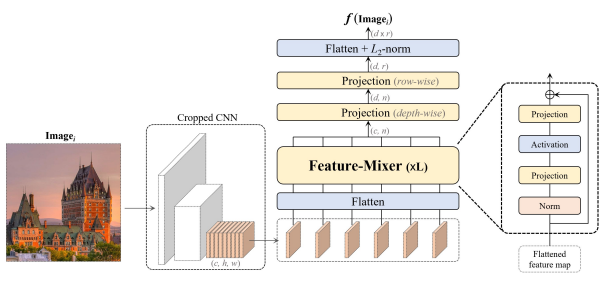
\includegraphics[scale=0.7]{pics/Proposal/mixvpr.png}
    \caption{Tổng quát quá trình xử lý ảnh của MixVPR \cite{alibey2023mixvpr}}
\end{figure}
Với ảnh đầu vào là $I$, mô hình CNN cơ sở sẽ trích xuất ra được tập Feature Map có dạng $F \in R^{c \cdot h \cdot w}$ từ những lớp trung gian.
$$
F = CNN(I)
$$
Ở những phương pháp trước như NetVLAD \cite{arandjelović2016netvlad} và PatchNetVLAD \cite{hausler2021patchnetvlad}, những lớp Feature Map thuộc $F$ sẽ được xem như là một mô tả tương ứng với một miền tiếp nhận trong ảnh ban đầu. Ngược lại, MixVPR xem tensor $F$ như một tập các đặc trưng 2D có kích thước $h \cdot w$.
$$
F = \{X^{i}\}    i = \{1,...c\}
$$
với $X^{i}$ tương ứng với bản đồ kích hoạt thứ $i$ ở F. Ở cách biểu diễn này, mỗi Feature Map không chỉ đại diện cho một miền tiếp nhận trong ảnh mà sẽ chứa một loại thông tin đặc thù cho toàn bộ ảnh. $X^{i}$ sau đó sẽ được định dạng lại thành ma trận một chiều, có được $F \in R^{c \cdot n}$ với $n = h*w$.

Sau đó, dữ liệu sẽ được đưa qua khối Feature Mixer, gồm $L$ những lớp mạng MLP. Những lớp này sẽ nhận vào từng Feature Map $X^{i}$ một chiều và tích hợp thông tin về mối liên kết giữa các giá trị của $X^{i}$ lên chính nó thông qua cách sau:
$$
X^{i} \leftarrow Norm(X^{i})
$$

$$
X^{i} \leftarrow W_2(\sigma(W_1 X^{i}))
$$
với $W_1$ và $W_2$ là trọng số của hai lớp liên kết đầy đủ, cấu tạo nên MLP và $\sigma$ là hàm tạo sự phi tuyến tính cho quá trình xử lý(ReLU). Kỹ thuật nối tắt được sử dụng để nối đầu vào đã qua lớp chuẩn hóa với đầu ra nhằm giúp độ dốc trong quá trình huấn luyện có thể được truyền tải dễ hơn, cải thiện quá trình huấn luyện.

Mục đích của việc sử dụng Feature Mixer là để tận dụng khả năng tổng hợp thông tin từ dữ liệu của các lớp kết nối đầy đủ, thay vì học trên những đặc trưng cục bộ trên ảnh và sử dụng cơ chế tập trung. Ngoài ra, Feature Mixer cũng sẽ trả về kết quả có định dạng như cũ, thay vì có đầu ra giảm dần như những phương pháp tổng hợp dạng phân cấp(kim tự tháp) như trước đây, để mỗi nơ-ron đều có thể biết được thông tin của toàn bộ ảnh. Những lớp MLP trong khối Feature Mixer sẽ giúp tích hợp thông tin trên toàn bộ ảnh qua mỗi lần xử lý.

Mỗi khối Feature Mixer sau khi xử lý xong từng Feature Map trong tập $F \in R^{c \cdot n}$, sẽ ghép kết quả lại, tạo thành $Z \in R^{c \cdot n}$ với cùng kích thước trước khi được đưa vào khối Feature Mixer kế tiếp. Quá trình này có thể được miêu tả bằng công thức sau:
$$
Z = FM_L(FM_{L-1}(\dots FM_1(F)))
$$
Số chiều của $Z$ thường sẽ rất cao do có định dạng được giữ nguyên so với $F$. Để giúp giảm bớt số chiều của $Z$ lại sau khi qua khối Feature Mixer, hai lớp kết nối đầy đủ sẽ được sử dụng để tổng hợp giữa các kênh với nhau và sau đó là giữa các giá trị trong từng kênh. Tác vụ này thực hiện việc tổng hợp có chọn lọc nhằm điều khiển được kích thước của giá trị đầu ra.

Đầu tiên, dữ liệu sẽ được tổng hợp số kênh để biến định dạng của $Z$ từ $R^{c \cdot n}$ thành $R^{d \cdot n}$.
$$
Z' = W_d(Transpose(Z))
$$
với $W_d$ là trọng số của lớp kết nối đầy đủ đầu tiên.

Sau đó, giá trị trên từng kênh sẽ được tổng hợp lại, từ định dạng $R^{d \cdot n}$ thành $R^{d \cdot r}$.
$$
O = W_r(Transpose(Z'))
$$
với $W_r$ là trọng số của lớp kết nối đầy đủ thứ hai.

Kết quả $O$ cuối cùng, có định dạng là $R^{d \cdot r}$, sẽ được ép thành một chiều và chuẩn hóa theo L2 như những phương pháp VPR khác \cite{arandjelović2016netvlad,berton2022rethinking}. Cuối cùng, từ ảnh đầu vào $I$, mô hình sẽ trả về một đoạn mã hóa biểu diễn cho nội dung của ảnh. Đoạn mã hóa này sau đó có thể được dùng để so sánh với giá trị mã hóa của những hình khác nhằm tìm ảnh có độ tương đồng cao nhất với $I$.

\subsubsection*{Chi tiết hiện thực phương pháp}
\textbf{Cấu trúc:} Phương pháp tổng hợp sử dụng mô hình MixVPR sẽ được hiện thực trên framework PyTorch. Mô hình CNN cơ sở của MixVPR sẽ được cắt ở lớp áp cuối của mô hình ResNet. Dữ liệu đầu vào cho MixVPR sẽ là một tập các Feature Map có kích thước 20x20. Thao tác tổng hợp trong khối Feature Mixer sẽ sử dụng lớp Linear được cung cấp bởi PyTorch, theo sau đó là một lớp ReLU để tạo tính phi tuyến tính. Với lớp chuẩn hóa, LayerNorm của PyTorch sẽ được sử dụng. Cuối cùng, đầu ra cuối cùng của khối Feature Mixer sẽ được tổng hợp xuống một chiều không gian biểu diễn nhỏ hơn sử dụng hai lớp kết nối đầy đủ giữa các kênh với nhau và giữa các giá trị trong mỗi kênh, chứng minh là MixVPR là một cấu trúc chỉ sử dụng MLP. Số khối Feature Mixer được sử dụng sẽ luôn được giữ là $L=4$ trừ khi được quy định khác.

\textbf{Huấn luyện:} Mô hình MixVPR được đánh giá trong bài nghiên cứu sẽ sử dụng mô hình ResNet \cite{he2016deep} đã được huấn luyện trên tập ImageNet \cite{krizhevsky2012imagenet} làm cơ sở. Sau đó, mô hình sẽ được huấn luyện trên tập dữ liệu GSV-Cities \cite{Ali_bey_2022}. Đối hàm mất mát, hàm Multi-Similarity Loss \cite{wang2019multi} do hàm đã được chứng mình là hỗ trợ cho ra kết quả tốt với tác vụ VPR \cite{Ali_bey_2022}. Kích thước của một batch sẽ có $P$ = 120 địa điểm, mỗi địa điểm được miêu tả bởi 4 ảnh, tạo thành một batch có kích thước 480 ảnh. Phương tối ưu giảm độ dốc ngẫu nhiên - SGD sẽ được sử dụng với quán tính - momentum là 0.9 với giá trị suy giảm trọng số - weight decay là 0.001. Tốc độ học - learning rate sẽ được khởi tạo với giá trị 0.05 và sẽ được chia 3 sau mỗi 5 chu kỳ - epoch. Cuối cùng, mô hình sẽ được huấn luyện tối đa 30 chu kỳ - epoch với đầu vào là ảnh đã được chỉnh xuống kích thước 320x320.

\textbf{Đánh giá:} Để đánh giá, 5 tiêu chuẩn sẽ được sử dụng. Pitts250k-test \cite{6618963}, bao gồm 8k ảnh truy vấn và 83k ảnh tham khảo, được thu thập từ Google Street View và Pitts30k-test \cite{6618963} là một tập con của Pitts250k bao gồm 8k ảnh truy vấn và 8k ảnh tham khảo. Cả 2 tập dữ liệu Pittsburgh đều có những góc nhìn có độ lệch đáng kể. Tập dữ liệu SPED \cite{zaffar2021vpr} gồm 607 ảnh truy vấn và 607 ảnh tham khảo từ camera giám sát chứa những thay đổi lớn về độ sáng và về cảnh vật các mùa. MSLS \cite{warburg2020mapillary} được thu thập từ camera hành trình của xe hơi và cho rất nhiều góc nhìn đa dạng và sự thay đổi về độ sáng. Cuối cùng, Nordland \cite{zaffar2021vpr} là một tập dữ liệu chứa nhiều thử thách khi sử dụng ảnh thu thập được ở cả 4 mùa với camera được gắn trên tàu. Đơn vị đánh giá được sử dụng sẽ là recall@k, thể hiện tỷ lệ của truy xuất thành công trên tổng số lượng truy xuất. Một truy xuất hình sẽ được xem là thành công khi ảnh được truy xuất nằm trong vòng 25m xung quanh ảnh truy vấn.

\subsubsection*{Hiệu quả của phương pháp}
Khi so sánh trên những tập dữ liệu phản ánh môi trường thành thị, phương pháp sử dụng mô hình MixVPR đạt được kết quả vượt trội so với những mô hình SOTA đã được đề xuất trước nó, như CosPlace \cite{berton2022rethinking} và NetVLAD \cite{arandjelović2016netvlad}. Những tập dữ liệu được sử dụng đã bao quát hết những trường hợp có thể tác động xấu đến mô hình như góc nhìn đa dạng; thời tiết, mùa thay đổi; chênh lệch về độ sáng.

MixVPR cũng có khả năng giải quyết được những trường hợp mà những phương pháp trước gặp khó khăn như:
\begin{itemize}
    \item Kiến trúc lặp lại nhiều
    \item Góc nhìn thay đổi rõ rệt
    \item Đường chân trời
    \item Độ sáng chênh lệch lớn
    \item Gặp nhiều vật thể cản trở tầm nhìn
\end{itemize}
Tuy nhiên, mô hình vẫn sẽ gặp thất bại khi độ chênh lệch góc nhìn là quá lớn hoặc có quá nhiều vật cản.

\begin{figure}[H]
    \centering
    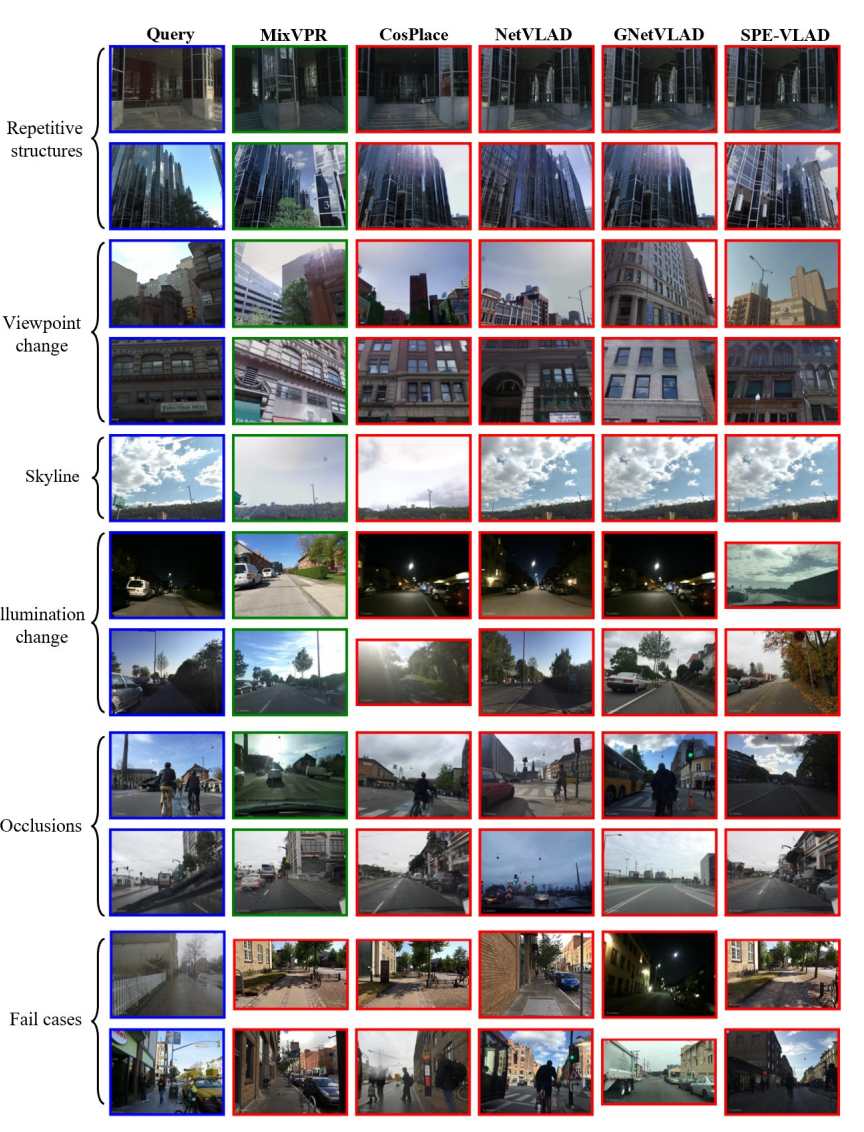
\includegraphics[scale=0.5]{pics/Proposal/fail.png}
    \caption{So sánh kết quả của những trường hợp khó của MixVPR và các phương pháp khác \cite{alibey2023mixvpr}}
\end{figure}

Với sự ra đời của AnyLoc \cite{keetha2023anyloc}, bài toán VPR trong những môi trường đa dạng hơn như trong nhà, trong hang động, trên bầu trời, hoặc trên mặt biển đã có một SOTA mới. Điều này là nhờ việc AnyLoc sử dụng mạng cơ sở DINO, một mạng Vision Transformer được huấn luyện bằng cơ chế tự giám sát để sinh ra những đặc trưng có giá trị với mọi tác vụ. Tuy nhiên, khi xét đến môi trường thành thị thì MixVPR vẫn có cho ra kết quả chính xác hơn AnyLoc. Số liệu cụ thể sẽ được trình bày bên dưới.

\begin{figure}[H]
    \centering
    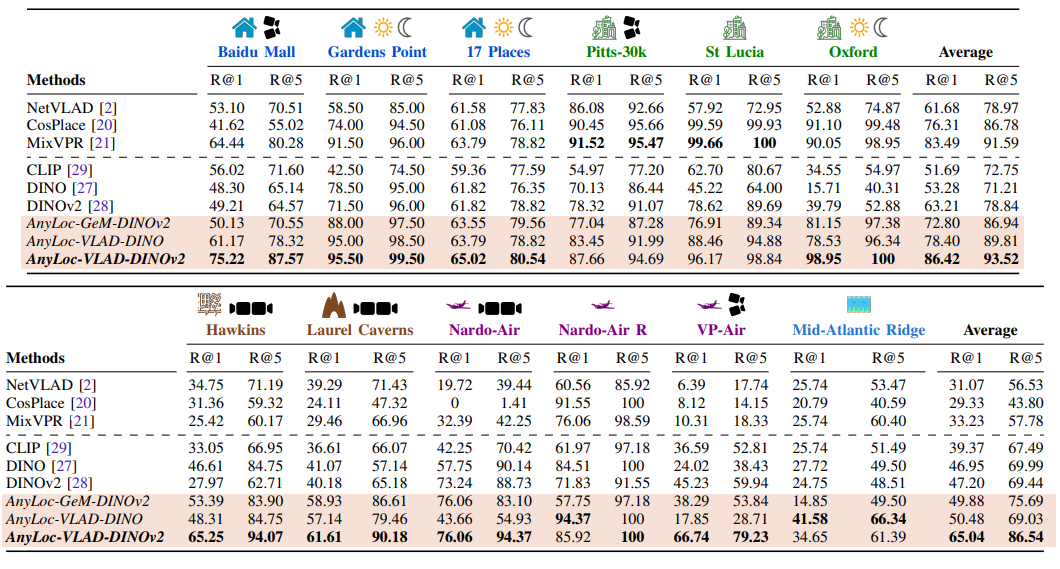
\includegraphics[scale=0.5]{pics/Proposal/anyloc.png}
    \caption{Kết quả của AnyLoc so sánh với những mô hình khác \cite{keetha2023anyloc}}
\end{figure}



\subsection{Mô hình tương quan 2D-2D của Map-free Relocalization \cite{arnold2022mapfree}}
\subsubsection*{Ý tưởng đằng sau mô hình}
Mô hình tương quan 2D-2D được đề xuất trong Map-free Relocalization thuộc nhóm những phương pháp sử dụng tìm kiếm cặp đặc trưng tương quan trong ảnh và xác định quy mô qua ước tính độ sâu. Phương pháp này sẽ giải quyết được điểm yếu của những phương pháp RPR là không nắm bắt được thông tin về hình học trong ảnh bằng cách sử dụng cách biểu diễn trung gian là ma trận thiết yếu. Dù kết quả của mô hình trong những môi trường có tập dữ liệu ảnh biểu diễn phân bố dày đặc là không quá vượt trội. Tuy nhiên, khi phân bố ảnh trong tập dữ liệu trở nên thưa hơn trong không gian đang xét thì phương pháp 2D-2D lại có kết quả vượt qua phương pháp 2D-3D và 3D-3D. 
\subsubsection*{Những bước xử lý của mô hình}

Với đầu vào là cặp ảnh $(I_0,I_1)$, những cặp đặc trưng tương quan giữa hai ảnh sẽ được xác định thành 2 tập là $(kpts_0, kpts_1)$ tương ứng với mỗi hình. Sau đó, ma trận thiết yếu giữa 2 ảnh sẽ được ước tính dựa vào giải thuật 5 điểm \cite{nister2004efficient} cùng với MAGSAC++ \cite{barath2020magsac++} dựa trên 2 tập điểm tương quan đã được xác định. Ma trận thiết yếu sau đó sẽ được phân giải thành ma trận thể hiện góc quay chênh lệch, $R \in SO(3)$ và vector đơn vị độ lệch về vị trí giữa hai ảnh, $\hat{t} \in R^{3}, \lvert \hat{t} \rvert = 1$.

Các cặp điểm tương quan giữa hai ảnh thỏa ma trận thiết yếu sẽ được chiếu lên không gian 3D qua độ sâu của ảnh. Với mỗi cặp điểm $(p_0,p_1)$, một tỷ lệ $s$ có thể được xác định bằng công thức:
$$
\begin{aligned}
    s=\underset{s^*}{\arg \min }\left\|R p_A+s^* \cdot \hat{t}-p_B\right\|_2 .
\end{aligned}
$$

\begin{figure}[H]
    \centering
    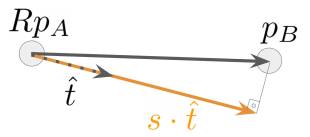
\includegraphics[scale=0.8]{pics/Proposal/reprojection.png}
    \caption{Hình minh họa cho việc chiếu điểm $p_0$ qua vector góc quay $R$ và vector độ lệch đơn vị $\hat{t}$ cùng với tỷ lệ $s$ để tối thiểu khoảng cách \cite{arnold2022mapfree}}
\end{figure}


Mỗi cặp tương quan sẽ trả về một tỷ lệ $s$ cho vector đơn vị độ lệch. Vòng lặp RANSAC sẽ được sử dụng để loại bỏ những trường hợp ngoại lệ sinh ra từ việc ước lượng độ sâu sai lệch. Sau đó, giá trị $s$ có số cặp điểm hợp lệ lớn nhất sẽ được chọn để kiếm được vector độ lệch. Một cặp điểm sẽ được coi là hợp lệ nếu khoảng cách giữa hai điểm sau phép chiếu nhỏ hơn một giá trị nhất định. Trong bài nghiên cứu, giá trị 10cm được chọn.

\subsubsection*{Chi tiết hiện thực phương pháp}

\textbf{Cấu trúc:} Tác vụ tìm kiếm tương quan giữa hai ảnh sẽ có thể lựa chọn giữa phương pháp truyền thống như SIFT, hoặc những phương pháp theo hướng tiếp cận học sâu gần đây hơn như SuperPoint+SuperGlue \cite{sarlin2020superglue} và LoFTR \cite{sun2021loftr}. Tác vụ tính độ sâu đơn ảnh sẽ được phân thành hai trường hợp là bên trong nhà và ngoài trời. Với những tập dữ liệu trong nhà, mô hình DPT \cite{ranftl2021vision} được huấn luyện trên tập dữ liệu NYUv2 \cite{silberman2012indoor} PlaneRCNN \cite{liu2019planercnn} được huấn luyện trên tập dữ liệu ScanNet \cite{dai2017scannet}. Với trường hợp ngoài trời, mô hình DPT \cite{ranftl2021vision} được huấn luyện trên tập KITTI sẽ được sử dụng \cite{geiger2012we}.

\textbf{Đánh giá:} Để đánh giá hiệu quả của mô hình trong tác vụ định vị trực quan, một số tiêu chí cơ bản đã được đưa ra như độ lệch về góc quay, độ lệch về vị trí của máy ảnh, cũng như một sai số mới được đưa ra trong bài nghiên cứu, sai số phản chiếu của điểm 3D ảo - VCRE, được lấy cảm hứng từ sai số phản chiếu của những điểm tương ứng - DCRE \cite{wald2020beyond}. Cụ thể, với giá trị dự đoán $(R,t)$ và giá trị thực $(R_{gt},t_{gt})$, các sai số sẽ được xác định như sau:
\begin{itemize}
    \item Sai số về góc quay, $\measuredangle(R,R_{gt})$, sẽ được tính là độ chênh lệch giữa góc quay được dự đoán và góc quay thực tế.
    \item Sai số về độ lệch máy quay sẽ được tính là khoảng cách Euclidian giữa cặp vị trí $(c,c_{gt})$ được tính theo công thức $c=-R \intercal t$.
    \item Sai số phản chiếu của điểm 3D ảo sẽ được dùng để đánh giá độ lệch của những vật thể trong không gian thực tế ảo. Giá trị thực $(R_{gt},t_{gt})$ và giá trị dự đoán $(R,t)$ sẽ được dùng để chiếu những điểm 3D ảo, lên hệ tọa độ của camera truy vấn. Giá trị VCRE sẽ được xác định theo công thức
    $$
    \operatorname{VCRE}=\frac{1}{|\mathcal{V}|} \sum_{\mathbf{v} \in \mathcal{V}}\left\|\pi(\mathbf{v})-\pi\left(T T_{\mathrm{gt}}^{-1} \mathbf{v}\right)\right\|_2 \quad \text { với } T=[R \mid t]
    $$

    với $\pi$ là phép chiếu từ không gian camera lên ảnh, $\mathcal{V}$ là một tập các điểm 3D, đại diện cho những vật thể ảo. $\mathcal{V}$ là một lưới điểm 3D, (chiều cao là 4, chiều rộng là 7 và chiều sâu là 7), cách nhau 30cm và có độ dịch là 1.8m dọc theo trục của máy ảnh. Giá trị sai số của phép phản chiếu sẽ được so sánh với đường chéo của ảnh.
    \item Độ tin cậy của dự đoán cũng là một tiêu chí được đánh giá. Giá trị này cho phép mô hình có thể phát hiện và loại bỏ những dự đoán không đáng tin cậy. Giá trị này sẽ được xác định bằng số lượng cặp điểm tương quan thỏa ma trận thiết yếu được chọn trên tổng số cặp điểm tương quan xác định bởi mô hình ghép đặc trưng. Với một ngưỡng tin cậy nhất định, tỷ lệ dự đoán đáng tin cậy - ratio of confident estimate, sẽ được xác định là tỷ lệ của những ảnh truy vấn có độ tin cậy vượt qua ngưỡng.
    \item Độ chính xác của mô hình sẽ là tỷ lệ của những ảnh đáng tin cậy có sai lệch giữa giá trị dự đoán và giá trị thực dưới một ngưỡng nhất định (độ lệch vị trí và góc quay) hoặc có sai số phản chiếu chấp nhận được trên tổng số ảnh.
\end{itemize}

Tập dữ liệu 7Scenes \cite{6619221} sẽ được sử dụng để xác định hiệu quả của mô hình tiêu chuẩn của Mapfree sẽ có hiệu quả như thế nào so với những phương pháp SOTA tại thời điểm đó, với số lượng ảnh tham khảo là rất nhiều. Ảnh hưởng của việc giảm số lượng ảnh tham khảo lên khả năng hoạt động của các mô hình cũng sẽ được ghi nhận lại. Tập dữ liệu Niantic được đề xuất trong cùng bài nghiên cứu cũng sẽ được sử dụng để đánh giá, nhằm xác định hiệu quả của các mô hình trong trường hợp chỉ có một ảnh tham khảo.

\subsubsection*{Hiệu quả của phương pháp}

\textbf{Tập dữ liệu 7Scenes \cite{6619221}}

\begin{figure}[H]
    \centering
    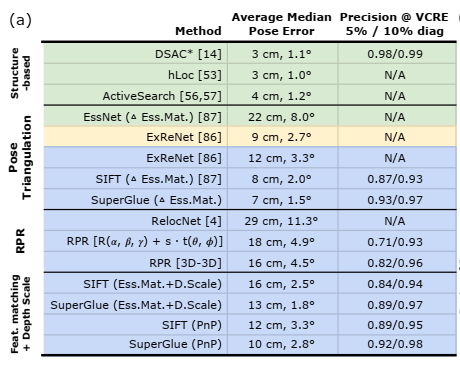
\includegraphics[scale=0.8]{pics/Proposal/all_7scene.png}
    \caption{Hiệu quả của những mô hình khi có đầy đủ ảnh tham khảo trên tập 7Scenes. Những phương pháp \textcolor{green}{xanh lá} sẽ phụ thuộc vào tập dữ liệu, phương pháp \textcolor{yellow}{vàng} được huấn luyện trên SUNCG \cite{song2017semantic} và \textcolor{blue}{xanh dương} trên tập ScanNet \cite{dai2017scannet}}
\end{figure}

Khi xét trên tập dữ liệu 7Scenes với tất cả các ảnh tham khảo, những phương pháp sử dụng biểu diễn 3D như DSAC* \cite{brachmann2021visual}, hLoc \cite{sarlin2019coarse}, ActiveSearch \cite{sattler2016efficient} có kết quả tốt nhất, tuy nhiên lại phụ thuộc vào quá trình tái tạo lại cấu trúc. Những phương pháp sử dụng phép đạc tam giác, sử dụng 5 ảnh tham khảo có kết quả cạnh tranh so với những phương pháp sử dụng biểu diễn 3D, được ký hiệu bằng $\triangle$. 

Để thực hiện bài toán định vị không cần biểu diễn, chỉ một ảnh tham khảo sẽ được sử dụng cho một truy vấn cho những phương pháp trong tập \textit{hồi quy vị trí tương đối} và \textit{ghép cặp đặc trưng + độ sâu ảnh}. Cả hai lớp phương pháp đều có kết quả bị xuống cấp, với phương pháp ghép cặp + độ sâu tốt hơn những phương pháp hồi quy tương đối. Tuy nhiên, các phương pháp thuộc các lớp vẫn có kết quả cạnh tranh, có thể được phần nào giải thích bởi việc truy xuất ảnh tốt và sự phân bố dày đặc của tập dữ liệu.

\begin{figure}[H]
    \centering
    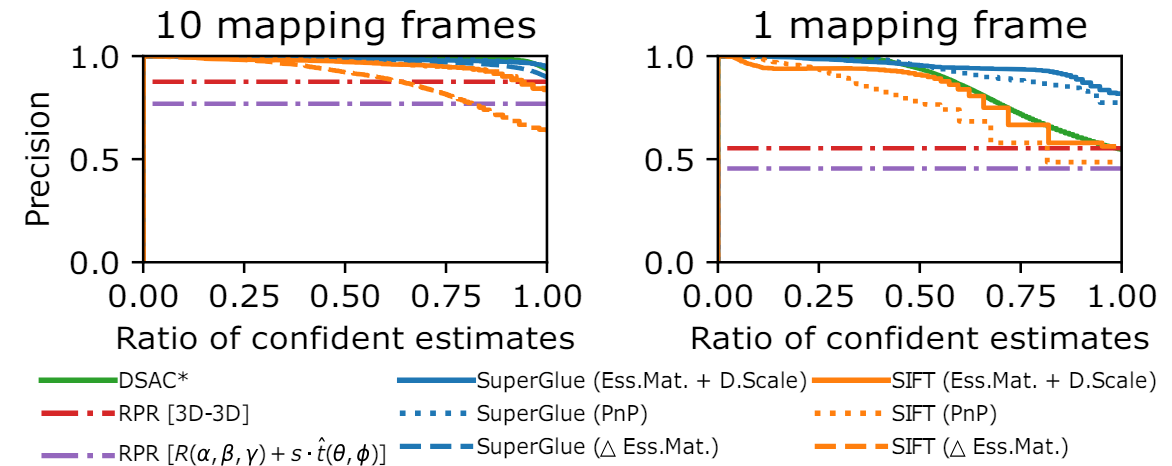
\includegraphics[scale=0.8]{pics/Proposal/partial_7scene.png}
    \caption{Hiệu quả của những mô hình khi tập 7Scenes chỉ có 10/1 ảnh tham khảo, đánh giá về độ chính xác và về số ảnh có sai số phản chiếu dưới ngưỡng.}
\end{figure}

Để có thể phản ánh một môi trường thực, nơi mà ảnh tham khảo truy xuất được cách xa đáng kể so với ảnh truy vấn, $K$ ảnh tham khảo mang nhiều thông tin nhất sẽ được chọn làm đại diện qua giải thuật gom cụm K-means.

Với việc so sánh độ chính xác ở hai kịch bản, ngưỡng chấp nhận về độ chính xác sẽ là $VCRE<10\%$ của đường chéo ảnh(80px). Khi ngưỡng tin cậy được hạ thấp, điều này làm cho tỷ lệ dự đoán đáng tin cậy tăng lên. Điều này làm độ chính xác giảm dần, do chứa những trường hợp có độ tin cậy không đủ cao. Trong trường hợp này, những mô hình 2D-2D, đặc biệt là mô hình sử dụng SuperGlue, có kết quả tốt hơn so với những mô hình còn lại, đặc biệt trong khoảng $0.5~1.0$. Ngoài ra, mô hình 2D-2D có thể tính ra vị trí và góc quay của hơn 50\% ảnh với VCRE < 40px.

Mô hình DSAC* vẫn có kết quả tốt nhất trong các mô hình. Tuy nhiên, phương pháp này lại phụ thuộc vào tập dữ liệu. Trong khi đó, những mô hình khác được huấn luyện trên tập ScanNet vẫn có kết quả tốt trên tập 7Scenes. Phương pháp sử dụng phép đạc tam giác cũng có kết quả cạnh tranh, tuy nhiên lại không thể hoạt động chỉ với một ảnh tham khảo. Những phương pháp ghép cặp + độ sâu có khả năng khái quát hóa tốt hơn những phương pháp RPR, như có thể thấy ở hiệu quả thấp hơn của những phương pháp hồi quy tương đối.

\textbf{Tập dữ liệu Niantic \cite{arnold2022mapfree}}

\begin{figure}[H]
    \centering
    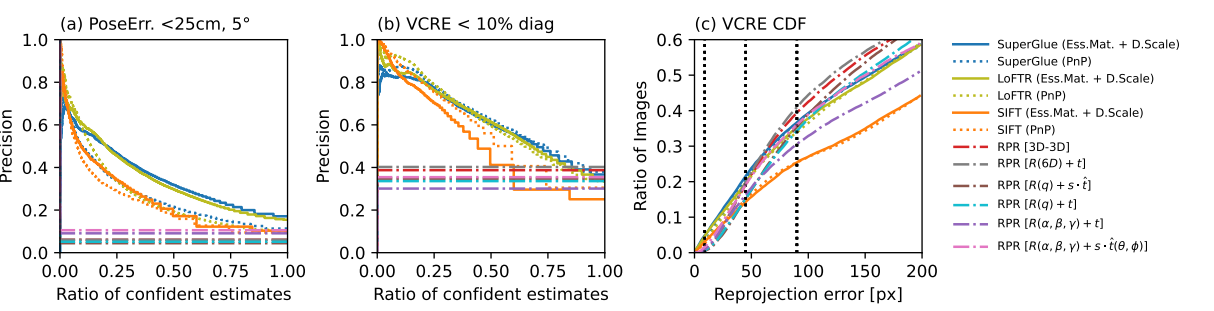
\includegraphics[scale=0.4]{pics/Proposal/all_niantic.png}
    \caption{Hiệu quả của các mô hình trên tập dữ liệu Niantic, xác định theo độ chính xác và số ảnh có sai số phản chiếu dưới ngưỡng}
\end{figure}

Qua kết quả thu được, tập dữ liệu Niantic có độ khó cao hơn đáng kể so với tập dữ liệu 7Scenes với mọi phương pháp. Điều này có thể thấy được rõ ràng từ kết quả của các mô hình. Trong tập dữ liệu Mapfree, những phương pháp 2D-2D tiếp tục có kết quả tốt. Tuy nhiên, ở những ngưỡng VCRE rộng hơn, những phương pháp RPR lại có kết quả tốt hơn. Điều này có thể giải thích được qua việc khi số cặp đặc trưng tương quan là không đủ chất lượng, độ lệch đơn vị vị trí được sinh ra có thể có sai số rất lớn so với thực tế. Vậy nên, những phương pháp RPR sẽ cho ra kết quả tốt khi ngưỡng chính xác rộng, nhưng lại có kết quả không tốt khi cần độ chính xác cao. Ngoài ra, những phương pháp RPR cũng không thể cung cấp độ tin cậy cho dự đoán của mô hình, hạn chế việc loại bỏ những dự đoán có khả năng sai cao.

\section{Mô hình kết hợp đề xuất}
Sau những nghiên cứu và tìm hiểu, nhóm quyết định đề xuất một mô hình kết hợp giữa MixVPR \cite{alibey2023mixvpr}và Map-free Relocalization \cite{arnold2022mapfree}. Gọi $I$ là ảnh mà người dùng chụp từ máy ảnh và sẽ được dùng làm ảnh truy vấn cho mô hình đề xuất của nhóm. Trước hết, mô hình sẽ nhận $I$ và truyền làm đầu vào cho MixVPR. Từ ảnh đầu vào $I$, sau khi qua các giai đoạn xử lý, MixVPR sẽ trả về một đoạn mã hóa biểu diễn cho nội dung của ảnh. Với đoạn mã hóa này, mô hình tiến hành so sánh với giá trị mã hóa của các ảnh trong cơ sở dữ liệu và tìm ra ảnh có sự tương đồng cao nhất với ảnh nhận vào $I$ gọi là $I_0$.

Bước tiếp theo, mô hình tiếp tục truyền cả ảnh nhận vào $I$ và ảnh được truy xuất $I_0$ cho mô hình tương quan 2D - 2D của Map-free Relocalization \cite{arnold2022mapfree}. Với đầu vào là cặp ảnh $(I, I_0)$, những cặp đặc trưng tương quan giữa hai ảnh sẽ được xác định tương ứng với mỗi hình. Sau đó, ma trận thiết yếu $E$ giữa 2 ảnh sẽ được ước tính dựa vào giải thuật 5 điểm \cite{nister2004efficient} cùng với MAGSAC++ \cite{barath2020magsac++} dựa trên 2 tập điểm tương quan đã được xác định. Ma trận thiết yếu sau đó sẽ được phân giải thành ma trận thể hiện góc quay chênh lệch và một véc-tơ thể hiện độ dịch vị trí thống nhất. Từ các thông tin đã nhận, mô hình tiến hành một bước chiếu ngược 3D để tính toán giá trị tỷ lệ $s$ với mỗi cặp điểm tương quan 3D - 3D.

Giá trị $s$ với số cặp điểm hợp lệ lớn nhất được chọn. Từ giá trị $s$ này, kết hợp với vị trí tương đối đã có được từ việc tính toán và phân tách ma trận thiết yếu, ta sẽ có được vị trí tuyệt đối của ảnh nhận vào $I$.
\begin{figure}[H]
    \centering
    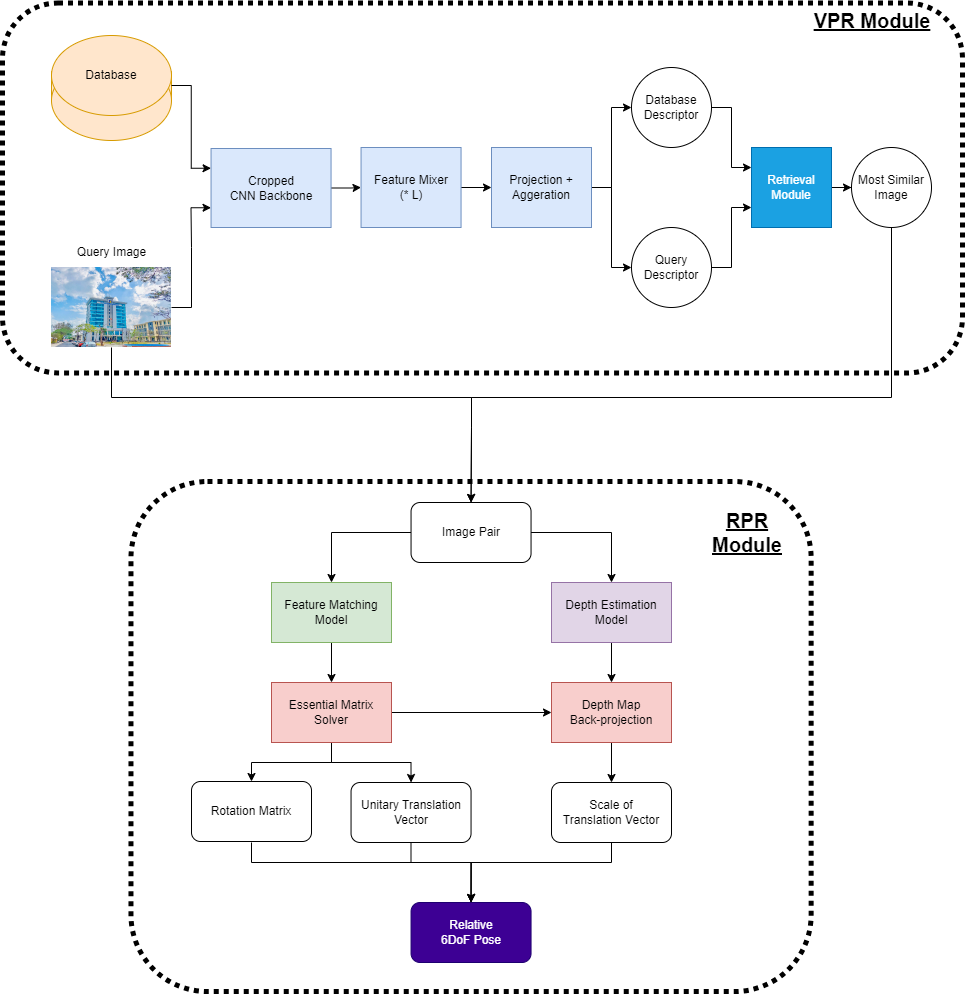
\includegraphics[scale=0.5]{pics/Proposal/models.png}
    \caption{Minh họa mô hình đề xuất}
\end{figure}